% Tarea 2, Modelado de sistemas (CE 1110). Documento iterativo:
% cada pregunta vive en secciones/pN_*.tex; compilar con ./compilar.sh
\documentclass[11pt,a4paper]{article}
% spanish.ldf no viene en todas las instalaciones; si falta, se usa el locale .ini.
\IfFileExists{spanish.ldf}
  {\usepackage[spanish,es-noshorthands,es-tabla]{babel}}
  {\usepackage{babel}\babelprovide[import,main]{spanish}
   \setlocalecaption{spanish}{table}{Tabla}}
% Las magnitudes ya incluyen su espacio antes del signo de porcentaje.
\ifdefined\spanishplainpercent\spanishplainpercent\fi
\usepackage[utf8]{inputenc}
\usepackage[T1]{fontenc}
\usepackage{lmodern}
\usepackage[margin=2.2cm]{geometry}
\usepackage{amsmath,amssymb}
\usepackage{booktabs,tabularx,array,enumitem}
\usepackage{graphicx}
\usepackage[table]{xcolor}
\usepackage{caption,subcaption}
\usepackage{placeins}
\usepackage{pgfplots}
\pgfplotsset{compat=1.18}
\usepgfplotslibrary{groupplots}
\usepackage[numbers]{natbib}
\usepackage{hyperref}
\hypersetup{colorlinks=true, urlcolor=blue!65!black, linkcolor=black, citecolor=black}
\usepackage{url}

\setlist{nosep,leftmargin=*}
\renewcommand{\arraystretch}{1.15}
\graphicspath{{figuras/}}

% Ruta del firmware del proyecto, para listar el código real y no una copia.
\newcommand{\firmware}{../../firmware}

% siunitx no está instalado en todas las máquinas del grupo: unidad mínima.
\providecommand{\SI}[2]{\ensuremath{#1\,\mathrm{#2}}}
\providecommand{\si}[1]{\ensuremath{\mathrm{#1}}}
\pgfplotsset{/pgf/number format/use comma}

% Enunciado de cada pregunta, en cursiva antes de la respuesta.
\newcommand{\enunciado}[1]{\par\noindent\emph{#1}\par\medskip}
% Enlaces de YouTube (no listados): reemplazar aquí y se actualizan en todo el informe.
\newcommand{\videoPlanta}{\url{https://youtu.be/B1e7-cnYzO4}}
\newcommand{\videoCaracterizacion}{\url{https://youtube.com/shorts/y-FDs2-BfVk}}



\begin{document}
\begin{titlepage}
  \centering
  
\includegraphics[width=0.55\linewidth]{logo_tec.png}\par\vspace{1cm}
  {\large Escuela de Ingeniería en Computadores\par}\vspace{0.4cm}
  {\large CE 1110 Análisis de Señales Mixtas\par}\vspace{2cm}
  {\Huge\bfseries Tarea 2: Teoría\par}\vspace{0.4cm}
  {\LARGE Modelado de sistemas\par}\vspace{2.5cm}
  {\large\bfseries Profesor:\par}
  {\large Luis Alberto Chavarría Zamora\par}\vspace{1cm}
  {\large\bfseries Estudiantes:\par}
  {\large Nicolás Florez Jiménez, 2024086367\par
   Tamara Vanessa Cajiao Molina, 2024143333\par
   Santiago Robles Obando, 2022207100\par
   Santiago Boza Quiros, 2024174347\par}
  \vfill
  {\large II Semestre 2026\par 22 de noviembre\par}
\end{titlepage}

\tableofcontents
\clearpage

\section*{Sistema de referencia}
\addcontentsline{toc}{section}{Sistema de referencia}
Las respuestas se ejemplifican con el banco de frenado del Proyecto Grupal~2: un disco movido por
un motor CD, un freno de goma accionado por un servomotor MG90S, un sensor óptico TCRT5000 frente a
10 marcas del disco ($N=10$ pulsos por vuelta) y un ESP32. En el proyecto final, el motor lleva el
disco a una velocidad inicial $\omega_0$, se corta, y un PID mueve el servo para que la velocidad
siga una referencia decreciente, por ejemplo $\omega_\text{ref}(t)=\max\{\omega_0-a\,t,\,0\}$. El
freno solo puede quitar velocidad, por lo que el error se toma con signo, $e=\omega-\omega_\text{ref}$:
si $e>0$ el freno aprieta y si $e<0$ suelta.

\section{Respuesta al impulso y al escalón en el modelado}
\label{sec:p1}
\enunciado{¿Por qué es importante la respuesta al impulso y al escalón para modelar sistemas?
Ejemplifique cada una en su proyecto (20\,\%).}

La respuesta al impulso y al escalón son útiles a la hora de modelar sistemas ya que permiten
observar de qué forma reacciona un sistema ante un cambio conocido. Si se mide esta reacción a lo
largo del tiempo, se puede construir un modelo que prediga cómo se comportará el sistema ante
otras condiciones. En el proyecto actual, se aprovechan de la siguiente manera:

\begin{itemize}
  \item \textbf{Respuesta al impulso:} Se aproxima un impulso dando un toque breve al freno
  mientras el disco se encuentra girando y soltarlo inmediatamente después. Este comportamiento
  permite registrar la velocidad antes, durante y después del toque, además de observar el tiempo
  en que tarda en notarse el frenado, así como la velocidad que pierde el disco durante ese breve
  tiempo.
  \item \textbf{Respuesta al escalón:} En este caso se puede generar una respuesta al escalón
  haciendo girar el disco y luego aplicando un frenado y mantener esa presión fija. Esto permite
  como la velocidad responde ante esa presión fija mantenida a lo largo del tiempo.
\end{itemize}

Si se toman los mismos valores iniciales (velocidad) para ambas pruebas, y se comparan con una
prueba donde el disco gira sin frenado, se puede distinguir mejor el efecto que ejerce el frenado
sobre el sistema y por lo tanto generar un modelo del sistema que relacione la relación entre el
frenado y la velocidad del disco.

\section{Frecuencia de muestreo de un sistema de control continuo}
\label{sec:p2}
\enunciado{¿Cómo determinar la frecuencia de muestreo de un sistema de control continuo? Proponga
una frecuencia razonable para el proyecto suyo (15\,\%).}

\subsection{Criterios}
Un controlador digital observa la planta solo en los instantes $t_k=kT_s$ y mantiene su salida
constante entre ellos con un retenedor de orden cero (ZOH). El teorema de Nyquist garantiza que una
señal de banda limitada se pueda reconstruir, pero en control no basta: el ZOH equivale
aproximadamente a un retardo de $T_s/2$, que resta al margen de fase
\begin{equation}
  \Delta\varphi \approx \frac{\omega_c T_s}{2}\ \text{[rad]},
  \label{eq:fase_zoh}
\end{equation}
donde $\omega_c$ es la frecuencia de cruce del lazo~\cite{franklin1998digital,astrom1997computer}.
Además, las aproximaciones de $s$ que convierten el PID en una ecuación en diferencias solo son
fieles si $T_s$ es pequeño frente a las constantes de tiempo del lazo~\cite{ogata1996discreto}.
Por eso se usan reglas prácticas: muestrear de 10 a 40 veces el ancho de banda de lazo cerrado
($\omega_s\approx 20\,\omega_b$)~\cite{franklin1998digital}, mantener $\omega_c T_s$ entre 0,15 y
0,5, y tener de 4 a 10 muestras por tiempo de subida~\cite{astrom1997computer}. El periodo también
debe ser compatible con el actuador, el sensor y el tiempo de cálculo.

\subsection{Propuesta: $T_s=\SI{20}{ms}$ ($f_s=\SI{50}{Hz}$)}
Para un frenado de 1,5 a 4~s y un servo que tarda unos 0,1~s en girar 60°~\cite{mg90s}, un ancho
de banda de lazo cerrado razonable es $\omega_b\approx\omega_c\approx$ 4 a $\SI{5}{rad/s}$. La
Tabla~\ref{tab:ts} verifica el periodo propuesto.

\begin{table}[h]
\centering\small
\caption{Verificación de $T_s=\SI{20}{ms}$ con $\omega_c=\SI{4}{rad/s}$.}
\label{tab:ts}
\begin{tabularx}{\linewidth}{@{}>{\raggedright\arraybackslash}p{4cm}>{\raggedright\arraybackslash}X>{\raggedright\arraybackslash}p{3.4cm}@{}}
\toprule
Criterio & Cálculo & Resultado \\
\midrule
$\omega_s \gtrsim 20\,\omega_b$ & $\omega_s=2\pi/T_s=\SI{314}{rad/s}$ frente a $\SI{100}{rad/s}$ & Cumple \\
$\omega_c T_s \leq 0{,}5$ & $4\cdot 0{,}02 = 0{,}08$ & Cumple \\
Fase del ZOH, ec.~\eqref{eq:fase_zoh} & $0{,}08/2=\SI{0{,}04}{rad}$ & $2{,}3^\circ$, despreciable \\
Muestras por subida & $t_r\approx 2{,}2/\omega_b\approx\SI{0{,}5}{s}$; $0{,}5/0{,}02$ & 25 \\
Actuador & El servo lee un pulso cada 20~ms~\cite{mg90s} & Muestrear más rápido no se aplica \\
\bottomrule
\end{tabularx}
\end{table}

El periodo de control no depende de la velocidad máxima del disco, que solo sirve para validar el
sensor. La velocidad se mide por tiempo entre marcas y no contando marcas en una
ventana~\cite{petrella2007speed}: con $N=10$, contar en 20~ms daría una resolución de
$2\pi/(N T_s)=\SI{31{,}4}{rad/s}$, mientras que medir el intervalo con resolución de 1~µs da
$0{,}024\,\%$ a $\SI{150}{rad/s}$.

Se propone $T_s=\SI{20}{ms}$: cumple las reglas con margen y coincide con la trama del servo. La
caracterización de la pregunta~7 lo confirma: la constante de tiempo medida, $\tau=\SI{0{,}274}{s}$,
corresponde a unas 14 muestras por constante de tiempo.

\section{Implementación de un PID en un microcontrolador}
\label{sec:p3}
\enunciado{¿Cómo se implementa un sistema PID en un microcontrolador? ¿Por qué no se debe usar la
función delay como en Arduino? Muestre el código en un microcontrolador sin la función
delay.}

\subsection{De la ley continua a la ecuación en diferencias}
El PID continuo es
$u(t)=K_p e(t) + K_i\int_0^t e\,d\tau + K_d\,\dot e(t)$~\cite{astrom2006advanced}.
En el microcontrolador se evalúa una vez por periodo y cada término se discretiza por
separado. Se usa Euler hacia atrás, $s\approx(1-z^{-1})/T_s$, que es simple y estable para
cualquier $T_s$~\cite{astrom1997computer,ogata1996discreto}:
\begin{align}
  P[k] &= K_p\,e[k], \\
  I[k] &= I[k-1] + K_i T_s\,e[k], \label{eq:integral}\\
  D[k] &= \frac{T_f}{T_f+T_s}\,D[k-1] + \frac{K_d}{T_f+T_s}\big(\omega[k]-\omega[k-1]\big), \label{eq:derivada}\\
  u[k] &= \operatorname{sat}_{[u_\text{mín},\,u_\text{máx}]}\big(P[k]+I[k-1]+D[k]\big).
\end{align}
Cuando no hay saturación, el controlador equivale a
\begin{equation}
  C(z) = K_p + \frac{K_i T_s}{1-z^{-1}} + \frac{K_d\,(1-z^{-1})}{(T_f+T_s) - T_f z^{-1}}.
\end{equation}
El proyecto exige además las siguientes decisiones de implementación.
\begin{itemize}
  \item La derivada pura amplifica el ruido
  del encoder, por eso se aplica $K_d s/(T_f s+1)$ con $T_f\approx 2T_s$. Derivar $\omega$ en
  lugar de $e$ evita saltos cuando cambia la referencia~\cite{astrom2006advanced}.
  \item El mando se satura a los límites calibrados del freno, que van de la goma sin contacto al
  frenado máximo seguro.
  \item Como anti-windup se usa integración condicional (\emph{clamping}): si $u$ está en un límite
  y el error empuja hacia ese mismo límite, \eqref{eq:integral} no se actualiza. Con un freno
  unilateral esto es importante, porque cuando la referencia pide más frenado del posible, el integrador
  acumularía un mando que después mantiene el freno apretado aunque el disco ya esté por debajo
  de la curva, y el freno no puede devolver esa velocidad~\cite{astrom2006advanced,astrom2021feedback}.
  \item Los estados $I$, $D$ y $\omega[k-1]$ se borran al inicio de cada
  frenado para que los ensayos sean comparables.
\end{itemize}

\paragraph{Ganancias provisionales.}
Partiendo de la planta~\eqref{eq:planta_G} de la pregunta~5: como el frenado dura mucho menos
que $J_\text{eq}/b$, el polo en $-b/J_\text{eq}$ queda cerca del origen y, agregando el servo,
la planta del mando a la velocidad es aproximadamente un integrador con el polo del servo,
$G(s)\approx -a_\text{máx}/\big(s(\tau_\text{servo}s+1)\big)$, con $a_\text{máx}=K_f/J_\text{eq}$
por unidad de mando. El signo
negativo se compensa con la convención $e=\omega-\omega_\text{ref}$. Con
$a_\text{máx}\approx\SI{100}{rad/s^2}$, $K_p=0{,}04$ da un cruce
$\omega_c\approx K_p a_\text{máx}=\SI{4}{rad/s}$, el usado en la pregunta~2. El cero del PI se
coloca debajo del cruce, en $K_i/K_p=\SI{2}{rad/s}$ ($K_i=0{,}08$), y $K_d=5\times10^{-4}$ es
pequeño. Como el lazo resulta de tipo~2, sigue la rampa sin error en estado estacionario. Son
valores de partida que se rediseñarán con el modelo identificado.

\subsection{Estructura temporal: periodo fijo sin bloqueo}
El periodo $T_s$ usado para calcular $K_iT_s$, $K_d/T_s$ y los polos en $z$ tiene que ser el
periodo real. La implementación (Listados~\ref{lst:pid} y~\ref{lst:main}) separa tres
contextos~\cite{picosdk}:
\begin{enumerate}
  \item La interrupción del encoder (\texttt{gpio\_set\_irq\_enabled\_with\_callback}) se
  activa en ambos flancos y solo guarda \texttt{time\_us\_64()}, así que no se pierde ninguna marca.
  \item El temporizador periódico (\texttt{add\_repeating\_timer\_us(-20000, ...)}) usa un
  retardo negativo, que hace que el SDK programe cada llamado 20~ms después del \emph{inicio} del
  anterior, de modo que el tiempo de ejecución no se suma al periodo. En cada tic se mide
  $\omega$, se calcula $\omega_\text{ref}(kT_s)$, se ejecuta \texttt{pid\_paso}, se escribe el
  PWM del servo y se encola la muestra. Primero se lee y se actúa, y después se guarda el
  registro, para minimizar la latencia entre medición y mando.
  \item El bucle principal no tiene requisitos de tiempo. Lee la consola con
  \texttt{getchar\_timeout\_us(0)}, que no bloquea, y vacía la cola de telemetría por USB. Si la
  cola se llena se descarta telemetría y se cuenta, pero nunca se retrasa el control.
\end{enumerate}
El tiempo de ejecución de cada paso se registra (\texttt{ejecucion\_us}) para demostrar que es
mucho menor que $T_s$.

\subsection{¿Por qué no usar \texttt{delay()}?}
El patrón típico de Arduino \texttt{loop()\{ medir(); pid(); actuar(); Serial.println(...);
delay(20); \}} tiene tres problemas:
\begin{enumerate}
  \item El periodo real no es $T_s$. El ciclo dura $T_\text{delay}+T_\text{ejec}$, y
  $T_\text{ejec}$ varía con la ruta del código y, sobre todo, con la impresión serie: a
  115\,200~baudios, una línea CSV de unos 40 caracteres tarda $\approx\SI{3{,}5}{ms}$. Las
  ganancias discretas $K_iT_s$ y $K_d/T_s$ y la ubicación de los polos en $z$ quedan calculadas
  para un periodo que no es el real, y el \emph{jitter} añade ruido de muestreo no
  uniforme~\cite{astrom1997computer}.
  \item La base de tiempo deriva. Si la referencia se calcula como $\omega_0-a\,kT_s$
  con un contador de muestras, el error se acumula y la curva seguida resulta más lenta que
  la diseñada.
  \item Bloquea el procesador. Durante \texttt{delay()} el programa no atiende la
  consola, los botones, la telemetría ni una condición de seguridad, como cortar el freno si se
  pierde el encoder~\cite{arduinoblink}.
\end{enumerate}
Si se trabaja en Arduino, la alternativa es la temporización no bloqueante con
\texttt{millis()}/\texttt{micros()}~\cite{arduinoblink}. El instante siguiente se acumula
(\texttt{siguiente += TS}), en vez de tomarse desde el instante actual
(\texttt{siguiente = ahora + TS}), para no acumular deriva:
\begin{lstlisting}[caption={Patrón no bloqueante equivalente en Arduino.},label={lst:millis},numbers=none]
if ((int32_t)(micros() - siguiente) >= 0) {  // seguro ante desborde
    siguiente += TS_US;                       // sin deriva acumulada
    paso_de_control();                        // medir -> PID -> actuar
}
atender_serial_y_botones();                   // nunca se bloquea
\end{lstlisting}
En la Pico se prefiere el temporizador por hardware (Listado~\ref{lst:main}), porque además
garantiza el periodo aunque el bucle principal esté ocupado.

\lstinputlisting[caption={Módulo PID portable (\texttt{firmware/src/pid\_controller.c}), el mismo que usa la simulación.},label={lst:pid}]{\firmware/src/pid_controller.c}

\subsection{Evidencia \simulado}
Para comprobar el código sin el banco, \texttt{evidencias/simulacion\_pid.c} compila el mismo
\texttt{pid\_controller.c} contra una planta \emph{ilustrativa}:
$\dot\omega = -\omega/8 - 1{,}5 - 100\,b$, donde $b$ es la posición del servo, con
$\tau_\text{servo}=\SI{50}{ms}$ y una trama PWM de retardo. Integra a 0,1~ms y el control corre
a $T_s=\SI{20}{ms}$. Los parámetros son supuestos y no provienen de una identificación del banco. Las
figuras y métricas se regeneran con \texttt{./compilar.sh}.

\paragraph{Anti-windup.} La referencia pide \SI{140}{rad/s^2} durante 0,5~s, más de lo que el
freno puede dar ($\approx\SI{120}{rad/s^2}$), y luego \SI{25}{rad/s^2}
(Fig.~\ref{fig:aw}). Sin anti-windup el freno sigue apretado después de alcanzar la curva y el
disco cae cerca de \SI{20}{rad/s} por debajo; como el freno no puede acelerarlo, queda más de
1~s suelto ($u=0$) esperando a que la referencia lo alcance. Con clamping el IAE baja de \iaeAwNo{} a
\iaeAwSi{}~rad y la fracción de muestras saturadas pasa de \satAwNo{} a \satAwSi{}\,\%.

\begin{figure}[h]
\centering
\begin{tikzpicture}
\begin{groupplot}[group style={group size=1 by 2, vertical sep=0.6cm, x descriptions at=edge bottom},
  width=0.92\linewidth, height=4.6cm, xmin=0, xmax=4, grid=major, grid style={gray!20},
  legend style={font=\footnotesize, at={(0.99,0.97)}, anchor=north east}]
\nextgroupplot[ylabel={$\omega$ [rad/s]}]
  \addplot[black, dashed, thick] table[x=t, y=ref, col sep=comma] {evidencias/generado/aw_si.csv};
  \addlegendentry{$\omega_\text{ref}$}
  \addplot[blue!70!black, thick] table[x=t, y=omega, col sep=comma] {evidencias/generado/aw_si.csv};
  \addlegendentry{con anti-windup}
  \addplot[red!70!black, thick] table[x=t, y=omega, col sep=comma] {evidencias/generado/aw_no.csv};
  \addlegendentry{sin anti-windup}
\nextgroupplot[ylabel={$u$ [norm.]}, xlabel={$t$ [s]}, ymin=-0.05, ymax=1.1]
  \addplot[blue!70!black, thick, const plot] table[x=t, y=u, col sep=comma] {evidencias/generado/aw_si.csv};
  \addplot[red!70!black, thick, const plot] table[x=t, y=u, col sep=comma] {evidencias/generado/aw_no.csv};
\end{groupplot}
\end{tikzpicture}
\caption{\simulado{} Seguimiento con una referencia que satura el freno al inicio.}
\label{fig:aw}
\end{figure}

\paragraph{Temporizador frente a \texttt{delay()}.} Con la rampa alcanzable de
\SI{40}{rad/s^2}, el mismo PID se ejecuta con el temporizador ($T_s$ exacto) y con un bucle
\texttt{delay(20)} más un cálculo de 0,3~ms y una impresión serie de 2,5 a 4,5~ms
(Fig.~\ref{fig:delay}). El periodo real medio sube a \periodoDelay~ms (máximo
\periodoMaxDelay~ms). Como la referencia avanza con el contador de muestras, al final el
firmware está atrasado \desfaseDelay~ms respecto al reloj real y la desaceleración efectiva
baja a $\approx$\decelEfectivaDelay~rad/s$^2$. Respecto de la curva diseñada, el IAE pasa de
\iaeTimer{} a \iaeDelay~rad y el RMSE de \rmseTimer{} a \rmseDelay~rad/s. Como las ganancias y
el código son idénticos, la diferencia se debe solo a la temporización.

\begin{figure}[h]
\centering
\begin{tikzpicture}
\begin{groupplot}[group style={group size=2 by 1, horizontal sep=1.6cm},
  height=5cm, grid=major, grid style={gray!20},
  legend style={font=\footnotesize, at={(0.99,0.97)}, anchor=north east}]
\nextgroupplot[width=0.56\linewidth, xmin=0, xmax=4.5, xlabel={$t$ [s]}, ylabel={$\omega$ [rad/s]}]
  \addplot[black, dashed, thick] table[x=t, y=ref, col sep=comma] {evidencias/generado/timer.csv};
  \addlegendentry{$\omega_\text{ref}(t)$}
  \addplot[blue!70!black, thick] table[x=t, y=omega, col sep=comma] {evidencias/generado/timer.csv};
  \addlegendentry{temporizador}
  \addplot[red!70!black, thick] table[x=t, y=omega, col sep=comma] {evidencias/generado/delay.csv};
  \addlegendentry{\texttt{delay(20)}}
\nextgroupplot[width=0.42\linewidth, xlabel={muestra $k$}, ylabel={periodo real [ms]}, ymin=19, ymax=26]
  \addplot[blue!70!black, thick, domain=0:200] {20};
  \addplot[red!70!black, only marks, mark size=0.6pt] table[x=k, y=periodo_ms, col sep=comma] {evidencias/generado/periodos_delay.csv};
\end{groupplot}
\end{tikzpicture}
\caption{\simulado{} Izquierda: seguimiento de la rampa. Derecha: periodo entre muestras con \texttt{delay(20)} (rojo) frente al temporizador (azul).}
\label{fig:delay}
\end{figure}

\pendiente{Repetir ambas comparaciones en el banco cuando la planta esté armada (preguntas 6 y
7): registrar \texttt{ejecucion\_us}, el periodo real entre muestras y el seguimiento con la
planta física.}

\section{Diagrama de bloques del sistema completo}
\label{sec:p4}
\enunciado{Realice un diagrama de bloques del sistema completo, de una descripción en prosa de
todos los componentes tanto continuos como discretos (25\,\%).}
\pendiente{Pregunta 4 (25\,\%). Diagrama (TikZ o figura en \texttt{figuras/}) y prosa.
\emph{Continuo:} motor CD, disco con inercia $J$, fricción viscosa y de Coulomb, goma y
mecánica del servo. \emph{Discreto:} encoder con marcas de tiempo (ISR), estimación de
$\omega[k]$, generador de $\omega_\text{ref}[k]$, comparador, PID con saturación y
anti-windup, PWM del servo (ZOH, trama de 20 ms) y registro por USB. Indicar dónde está cada
frontera continuo/discreto (muestreo $T_s$ y retención).}

\section{Representación matemática y respuesta esperada sin controlador}
\label{sec:p5}
\enunciado{De una representación matemática del sistema según la teoría. Explique cómo debería
quedar la respuesta final de la planta (sin controlador) y algunos posibles valores que se puedan
extraer teóricamente}

\subsection{Representación matemática del sistema}
El sistema de frenado se modela como un disco en rotación que, después de alcanzar una velocidad
angular inicial $\omega_0$, deja de recibir torque de accionamiento del motor DC y desacelera por
efecto de la fricción. La planta tiene como entrada la acción del freno $u(t)$, aplicada mediante
una goma movida por un servomotor MG90S, y como salida la velocidad angular $\omega(t)$ del disco.
Según la segunda ley de Newton para sistemas rotacionales, la suma de torques es igual al momento
de inercia equivalente multiplicado por la aceleración angular~\cite{openstax_rotacion}:
\begin{equation}
  J_\text{eq}\,\frac{d\omega(t)}{dt} = \tau_m(t) - b\,\omega(t) - \tau_f(t)
  \label{eq:newton_rot}
\end{equation}
En esta expresión, $J_\text{eq}$ representa el momento de inercia equivalente
(\si{kg\cdot m^2}), $\tau_m$ el torque del motor (\si{N\cdot m}), $b$ el coeficiente de fricción
viscosa (\si{N\cdot m\cdot s/rad}) y $\tau_f$ el torque resistivo del freno (\si{N\cdot m}).
Durante la etapa de frenado se aproxima $\tau_m \approx 0$, aunque los elementos que permanecen
acoplados al eje siguen contribuyendo a la inercia y a las pérdidas mecánicas. Para obtener una
función de transferencia aproximada, se consideran variaciones pequeñas $\Delta\omega$ y
$\Delta u$ y se supone localmente $\Delta\tau_f \approx K_f\,\Delta u$. Sustituyendo en la
ecuación rotacional se obtiene la ecuación incremental, y posteriormente se aplica Laplace con
condiciones iniciales incrementales nulas:
\begin{gather*}
  J_\text{eq}\,\frac{d\,\Delta\omega(t)}{dt} + b\,\Delta\omega(t) = -K_f\,\Delta u(t) \\[4pt]
  (J_\text{eq}s + b)\,\Delta\Omega(s) = -K_f\,\Delta U(s)
\end{gather*}
\begin{equation}
  G(s) = \frac{\Delta\Omega(s)}{\Delta U(s)} \approx \frac{-K_f}{J_\text{eq}s + b}
  \label{eq:planta_G}
\end{equation}
El signo negativo indica que incrementar el frenado disminuye la velocidad. Esta función de
transferencia es una aproximación lineal alrededor de un intervalo de operación, no un modelo
válido para toda la detención, pues la fricción, la presión de la goma y el comportamiento del
servo pueden ser no lineales~\cite{ctms_motor}. Esta simplificación se adopta porque permite
estudiar la relación entre la acción de frenado y la velocidad mediante la transformada de
Laplace, y proporciona un punto de partida para el diseño del controlador PID. La validez de la
aproximación no se da por supuesta: posteriormente se comprobará mediante la comparación del
modelo con datos experimentales en MATLAB, delimitando las condiciones de operación en las que
resulte representativo.

\subsection{Respuesta esperada de la planta sin controlador}
Sin PID, el servomotor aplica una posición de frenado fija y no corrige los cambios de velocidad
medidos. Si durante esa prueba se aproxima el torque resistivo total como constante y positivo,
$\tau_\text{res}$, la ecuación de movimiento se simplifica a:
\begin{equation}
  J_\text{eq}\,\frac{d\omega(t)}{dt} = -\tau_\text{res}
  \label{eq:torque_constante}
\end{equation}
Despejando la derivada de la velocidad e integrando con la condición inicial
$\omega(0)=\omega_0$, se obtiene la respuesta temporal. Se impone además $\omega(t)\geq 0$, ya
que la acción del freno no invierte el sentido del movimiento:
\begin{gather*}
  \frac{d\omega}{dt} = -\frac{\tau_\text{res}}{J_\text{eq}}
  \quad\Longrightarrow\quad
  \omega(t) = \omega_0 - \frac{\tau_\text{res}}{J_\text{eq}}\,t
\end{gather*}
\begin{equation}
  \omega(t) = \max\left\{0,\ \omega_0 - \frac{\tau_\text{res}}{J_\text{eq}}\,t\right\}
  \label{eq:respuesta_lineal}
\end{equation}
Por lo tanto, se espera una curva de velocidad aproximadamente lineal y decreciente hasta llegar a
\SI{0}{rad/s}. Una mayor acción de frenado produciría una pendiente más negativa y un menor tiempo
de detención. En el prototipo real pueden observarse desviaciones respecto a esa recta debido al
rozamiento viscoso, la fricción seca y el retardo de aplicación del freno. Incluso sin ejercer
presión con la zapata, el disco eventualmente se detendría por las pérdidas mecánicas; por eso se
deben comparar las curvas con y sin frenado aplicado.

\subsection{Valores que pueden extraerse teóricamente}
Las magnitudes teóricas se expresan en función de los parámetros del sistema, sin asignarles
valores numéricos. En general, el momento de inercia de un cuerpo que gira alrededor de un eje se
calcula a partir de su distribución de masa. Para un disco macizo y homogéneo, de masa $m$ y radio
$R$, esta relación se simplifica a~\cite{openstax_rotacion}:
\begin{equation}
  J_\text{disco} = \int r^2\,dm
  \quad\Longrightarrow\quad
  J_\text{disco} = \frac{1}{2}\,mR^2
  \label{eq:inercia_disco}
\end{equation}
Si varios elementos giran alrededor del mismo eje, su inercia se incorpora al momento equivalente
mediante $J_\text{eq} = J_\text{disco} + \sum J_i$. Bajo la hipótesis de torque resistivo total
constante, es posible determinar simbólicamente la aceleración angular y el tiempo de detención:
\begin{equation}
  \alpha = -\frac{\tau_\text{res}}{J_\text{eq}}\,;\qquad
  t_\text{det} = \frac{J_\text{eq}\,\omega_0}{\tau_\text{res}}
  \label{eq:alfa_tdet}
\end{equation}
La velocidad inicial se expresa en rad/s mediante $\omega_0 = 2\pi\cdot\text{RPM}_0/60$. Las
ecuaciones de movimiento son generales para sistemas rotacionales; la expresión
$J_\text{disco} = \tfrac{1}{2}mR^2$ corresponde específicamente a un disco uniforme. En esta etapa
no se asignan valores reales a los parámetros: posteriormente se identificarán y ajustarán en
MATLAB utilizando mediciones experimentales de entrada y velocidad, y se validará la capacidad
predictiva del modelo.

\section{Construcción de la planta (puntos extra)}
\label{sec:p6}
\enunciado{Construya la planta del proyecto (solo no tiene controlador pero si el resto de
componentes) (40\,\% extra). Adjunte fotos y video de la construcción final.}

\puntosextra{Se construyó la planta completa y se muestra funcionando en lazo abierto en el
video \videoPlanta. Solo falta cerrar el lazo con el PID, que corresponde al Proyecto Grupal~2.}

\subsection{Componentes y conexiones}
La Tabla~\ref{tab:planta} resume la planta construida, que implementa los bloques de la
Fig.~\ref{fig:sistema}.

\begin{table}[h]
\centering\small
\caption{Componentes y conexiones de la planta construida.}
\label{tab:planta}
\begin{tabularx}{\linewidth}{@{}>{\raggedright\arraybackslash}p{3.5cm}>{\raggedright\arraybackslash}X>{\raggedright\arraybackslash}p{3.3cm}@{}}
\toprule
Componente & Función & Conexión \\
\midrule
Disco de MDF & Rueda frenada; 10 marcas negras equidistantes sobre fondo blanco & Eje del motor \\
Motor CD & Lleva el disco a la velocidad inicial & Salidas OUT1/OUT2 del L298N \\
Puente H L298N & Etapa de potencia del motor & ENA 25, IN1 26, IN2 33 \\
Fuente del motor & Alimenta el motor a través del puente & Bornes +12V y GND del L298N \\
Servo MG90S + goma & Freno: 120° liberado, 180° frenado & Señal en GPIO18 (PWM 50~Hz) \\
Sensor TCRT5000 & Un pulso por marca, 10 por vuelta & Salida en GPIO27, a 3,3~V \\
ESP32 (ESP-IDF 5.5) & Mide, registra y manda freno y motor & USB a la computadora \\
\bottomrule
\end{tabularx}
\end{table}

\subsection{Funcionamiento del sistema}
\begin{itemize}
  \item \textbf{Motor CD y puente H.} Un pin del ESP32 entrega 3,3~V y pocos miliamperios,
  insuficientes para el motor, así que el L298N conmuta la corriente de una \textbf{fuente externa}
  conectada a sus bornes de potencia. El ESP32 solo envía señales lógicas: IN1/IN2 fijan el sentido
  y ENA, con PWM de 1~kHz, fija el porcentaje de voltaje aplicado. Para frenar, ENA pasa a bajo y el
  motor queda en \emph{marcha libre}. Así el motor no frena el disco y la única acción de frenado es la
  de la goma, que es la que se quiere caracterizar.
  \item \textbf{Freno.} El MG90S es un servo de posición: recibe un pulso cada 20~ms cuyo ancho
  (500 a 2500~µs) fija el ángulo. A 120° la goma está separada del disco y a 180° lo presiona. El
  freno es unilateral, como se discutió en la pregunta~5: solo quita velocidad.
  \item \textbf{Sensor óptico.} El TCRT5000 detecta por reflexión el paso de cada marca negra. El
  ESP32 fecha un solo flanco por marca con una interrupción y calcula la velocidad por tiempo entre
  marcas (pregunta~2). Un filtro descarta los flancos separados por menos de 500~µs, que son rebotes
  del comparador del módulo y no marcas reales.
  \item \textbf{ESP32 y computadora.} El firmware del banco (\texttt{firmware/} del repositorio)
  recibe comandos por la consola serie desde la computadora: \texttt{FRENO} mueve el servo,
  \texttt{MOTOR} impulsa el disco y \texttt{ENSAYO} ejecuta el ensayo de la pregunta~7. Durante una
  captura envía una fila \texttt{tiempo\_ms, freno\_deg, velocidad\_rpm} cada 20~ms.
  \item \textbf{Alimentación y tierra común.} El motor y el servo consumen picos de corriente que
  harían caer el voltaje del ESP32. Por eso cada potencia va por su lado y todas las tierras se unen,
  para que las señales lógicas tengan la misma referencia.
\end{itemize}

\subsection{Video en lazo abierto}
El video \videoPlanta{} muestra la planta operando sin controlador: el motor acelera el disco, se
corta, y el servo aplica la goma con un ángulo fijo, mientras el ESP32 mide la velocidad.

\IfFileExists{figuras/planta.jpg}{%
\begin{figure}[h]
\centering
\includegraphics[width=0.8\linewidth]{planta.jpg}
\caption{Planta construida.}
\label{fig:planta}
\end{figure}}{}

\section{Caracterización por respuesta al escalón (puntos extra)}
\label{sec:p7}
\enunciado{Caracterice el sistema mediante la respuesta al escalón (40\,\% extra). Adjunte un vídeo
de la respuesta al escalón (ejecutando la planta en físico con ustedes explicando y su
funcionamiento en computadora, debe ser un solo vídeo).}

\begin{center}
\textbf{Video del ensayo y su análisis en MATLAB:} \videoCaracterizacion
\end{center}

\subsection{Método}
Se usa un escalón del freno porque se puede aplicar de forma limpia y repetible; un impulso ideal
no es realizable, así que la respuesta al impulso se obtiene del modelo identificado (pregunta~1).
El motor acelera el disco, se corta, y tras un tramo de giro libre el servo pasa en una sola orden
de 120° a 180° y se mantiene. El ESP32 registra cada 20~ms el tiempo, el ángulo ordenado y la
velocidad en un archivo CSV.

El script \texttt{visualizar\_ensayo.m} ajusta una recta a la velocidad en los 300~ms anteriores y
posteriores al escalón. La pendiente previa $a_0$ es la caída libre por fricción. Suponiendo que el
freno añade una aceleración que crece como $K\Delta u\,(1-e^{-t/\tau})$, la velocidad predicha es
\[
  \widehat v(t)=v(0)+a_0t+K\Delta u\bigl[t-\tau(1-e^{-t/\tau})\bigr],\qquad t\geq 0,
\]
y $K$ y $\tau$ se ajustan por mínimos cuadrados hasta que el disco se detiene. El modelo
resultante, del ángulo del freno al cambio de velocidad respecto a la caída libre, es
\begin{equation}
  G(s)=\frac{K}{s(\tau s+1)},
  \label{eq:modelo_escalon}
\end{equation}
cuya respuesta al impulso se calcula con \texttt{tf} e \texttt{impulse} de MATLAB.

\subsection{Resultados}
El ensayo presentado (\texttt{escalon\_02}) tiene 500 muestras sin pérdidas. La
Fig.~\ref{fig:escalon02} muestra el escalón, la velocidad medida y el modelo ajustado, y la
Tabla~\ref{tab:caracterizacion} resume los resultados.

\begin{figure}[h]
\centering
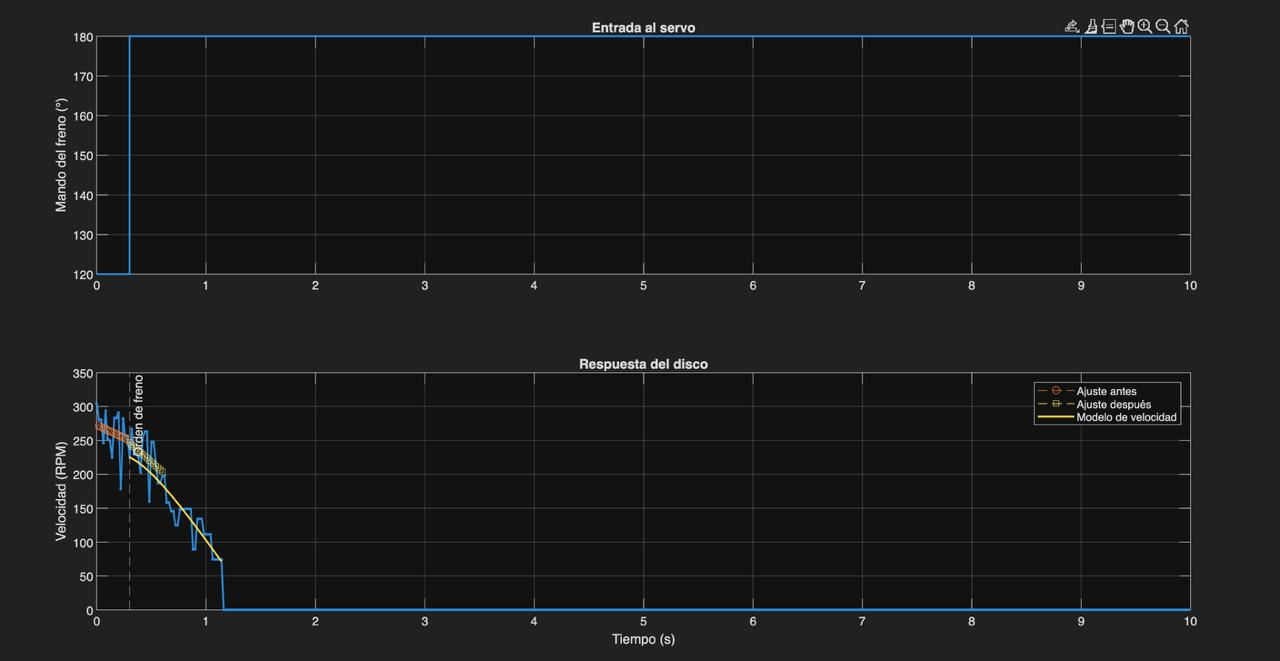
\includegraphics[width=\linewidth]{matlab_escalon_02.jpg}
\caption{Ensayo \texttt{escalon\_02}: orden al servo (arriba) y velocidad medida, rectas de
300~ms y modelo ajustado (abajo).}
\label{fig:escalon02}
\end{figure}

\begin{table}[h]
\centering\small
\caption{Resultados de la caracterización.}
\label{tab:caracterizacion}
\begin{tabular}{@{}lr@{}}
\toprule
Magnitud & Valor \\
\midrule
Velocidad al cortar el motor & $\approx 300$~RPM \\
Escalón $\Delta u$ & $120^\circ\to 180^\circ$ en $t=0{,}301$~s \\
Pendiente antes del freno & $-76{,}4$~RPM/s \\
Pendiente después del freno & $-142{,}9$~RPM/s \\
Ganancia $K$ & $-2{,}58$~(RPM/s)/grado \\
Constante de tiempo $\tau$ & $0{,}274$~s \\
RMSE del modelo & $25{,}0$~RPM \\
Detención del disco & $t\approx 1{,}14$~s \\
\bottomrule
\end{tabular}
\end{table}

Con estos valores,
\[
  G(s)=\frac{-2{,}58}{s\,(0{,}274\,s+1)}\ \frac{\text{RPM}}{\text{grado}},\qquad
  h(t)=-2{,}58\,\bigl(1-e^{-t/0{,}274}\bigr)\ \text{RPM},
\]
y la Fig.~\ref{fig:impulso02} muestra la respuesta al impulso obtenida con \texttt{impulse}.

\begin{figure}[h]
\centering
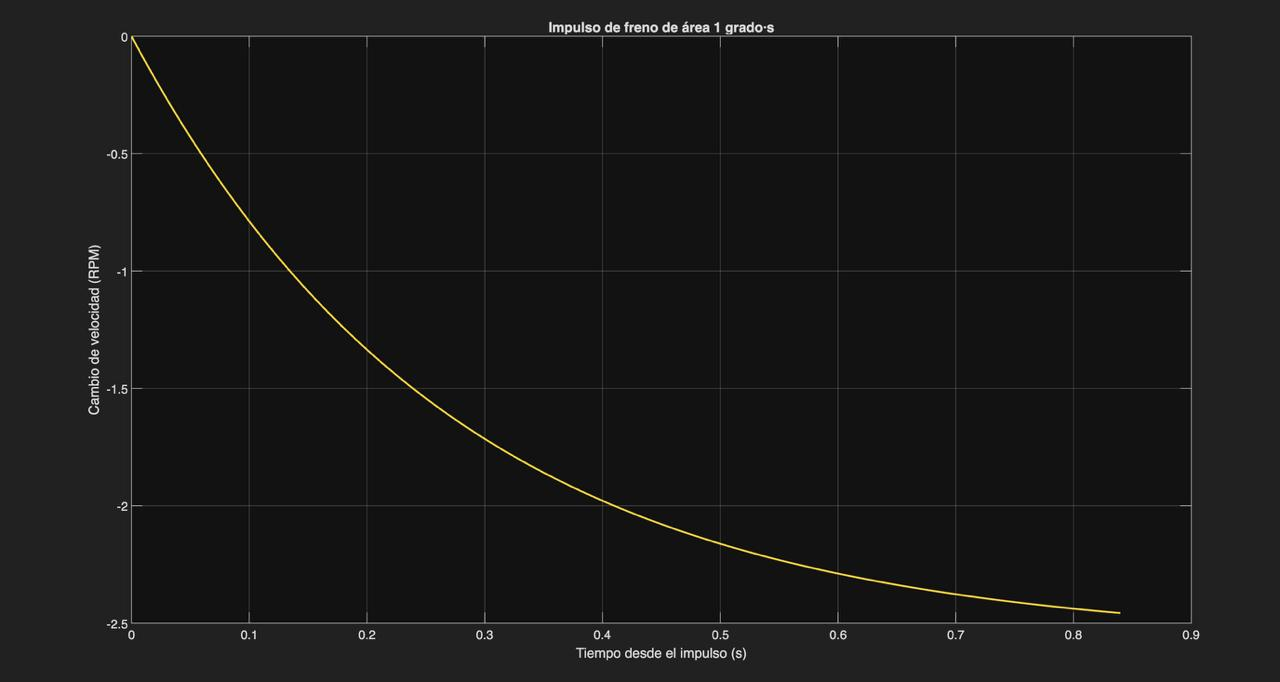
\includegraphics[width=0.8\linewidth]{matlab_impulso_02.jpg}
\caption{Respuesta al impulso del modelo identificado (impulso de 1 grado$\cdot$s).}
\label{fig:impulso02}
\end{figure}

\subsection{Análisis}
El freno casi duplica la desaceleración, de $-76$ a $-143$~RPM/s, y $K<0$ confirma que más ángulo
de freno quita velocidad. El resultado es coherente con el modelo de la pregunta~5: la caída libre
corresponde a los términos de fricción, que el método resta, y el efecto del freno no es
instantáneo sino que crece con $\tau=0{,}27$~s, que incluye el recorrido del servo y el tiempo de
contacto de la goma. Si $\tau\to 0$, la ec.~\eqref{eq:modelo_escalon} se reduce a la forma de la
pregunta~5 con $K=-K_f/J_\text{eq}$. El RMSE de 25~RPM proviene principalmente del ruido del
sensor, que produce saltos entre muestras. El modelo es local: es válido cerca de 300~RPM y para
este escalón, y debe validarse con otros ensayos antes de diseñar el PID.


\appendix
\section{Programas del microcontrolador}
\label{sec:codigo}
Los programas completos se entregan en el archivo comprimido, en la carpeta
\texttt{programas\_microcontrolador/}, y están en el repositorio del grupo. La
Tabla~\ref{tab:programas} indica qué programa corresponde a cada pregunta. Los listados de este
anexo son los del programa de la pregunta~3; el módulo PID está en el Listado~\ref{lst:pid}.

\begin{table}[h]
\centering\small
\caption{Programas por pregunta (rutas dentro del comprimido).}
\label{tab:programas}
\begin{tabularx}{\linewidth}{@{}>{\raggedright\arraybackslash}p{2.6cm}>{\raggedright\arraybackslash}p{6.2cm}>{\raggedright\arraybackslash}X@{}}
\toprule
Pregunta & Archivo & Contenido \\
\midrule
3 (PID sin \texttt{delay}) & \texttt{pregunta3\_pid/main\_tarea2.c} & Lazo con \texttt{esp\_timer}, ISR del sensor y telemetría (Listado~\ref{lst:main}) \\
 & \texttt{pregunta3\_pid/pid\_controller.c/.h} & PID discreto con anti-windup (Listados~\ref{lst:pid} y \ref{lst:pidh}) \\
 & \texttt{pregunta3\_pid/estimador\_velocidad.c}, \texttt{conversion\_freno.c} & Velocidad por tiempo entre marcas y grados a pulso del servo \\
6 y 7 (planta y ensayo) & \texttt{registrador\_banco/src/aplicacion.c} & Comandos \texttt{FRENO}, \texttt{MOTOR}, \texttt{ENSAYO} y registro cada 20~ms \\
 & \texttt{registrador\_banco/src/} (resto) & Sensor, servo, motor y protocolo serie \\
 & \texttt{registrador\_banco/sdkconfig.ensayo} & Pines y calibración usados en el ensayo \\
\bottomrule
\end{tabularx}
\end{table}

\lstinputlisting[caption={Lazo de control sin \texttt{delay()} para el ESP32 (\texttt{main\_tarea2.c}).},label={lst:main}]{codigo/main_tarea2.c}

\lstinputlisting[caption={Interfaz del PID (\texttt{pid\_controller.h}).},label={lst:pidh}]{\firmware/include/pid_controller.h}

\section{Videos y evidencias}
\label{sec:videos}
\begin{tabularx}{\linewidth}{@{}>{\raggedright\arraybackslash}p{6cm}X@{}}
\toprule
Evidencia & Enlace (YouTube, no listado) \\
\midrule
Planta en lazo abierto: impulso y frenado (pregunta 6) & \videoPlanta \\
Ensayo al escalón en el banco, captura del CSV y análisis en MATLAB (pregunta 7) & \videoCaracterizacion \\
\bottomrule
\end{tabularx}

\medskip
Datos y programas del ensayo en el repositorio: \texttt{experimentos/datos/escalon\_02.csv} y
su \texttt{.json}, \texttt{experimentos/consola\_banco.py} (captura) y
\texttt{matlab\_modelado/visualizar\_ensayo.m} (análisis).


\phantomsection\addcontentsline{toc}{section}{\refname}
\bibliographystyle{IEEEtran}
\bibliography{referencias}
\end{document}
